%%%%%%%%%%%%%%%%%%%%%%%
%% q-mem.tex
%%%%%%%%%%%%%%%%%%%%%%%

We now directly assess the cubic code as a self-correcting quantum memory.
The results in this chapter depend on previous chapters.
In Chapter~\ref{chap:consq-no-strings} 
we have found an energy barrier to isolate a nontrivial charge.
It implies that nontrivial charges are localized in their original position where they are created.
It suggests further that geometrically localized defects would form a neutral cluster,
and the annihilation of them would not likely cause any undetected logical error.
The renormalization group decoder and the threshold theorem 
in Chapter~\ref{chap:RG-decoder} have been motivated by this intuition.
In this chapter, we show that 
the performance of the RG decoder against thermal errors
matches our expectation, too.
We prove that if the no-strings rule is satisfied,
then the memory time grows as a power law 
$L^{c\beta}$ where $\beta$ is the inverse temperature of the heat bath.
The bound is valid when the system size is small enough $L \le e^{c' \beta}$.
Note that our analysis does not tell anything conclusive for the system in thermodynamic limit.

A few remarks can be made to the validity regime $L \le e^{c' \beta}$.
It is reasonable to expect that the no-strings rule and a good decoder
would be sufficient to guarantee that the memory time increases with the system size.
However, when the entropy is considered, the situation is more complicated.
From the degeneracy formula of the cubic code in Chapter~\ref{chap:cubic-code},
we know that there are system sizes where the number $k$ of encoded qubits is 2.
Since the cubic code has exactly one $X$-type stabilizer generator $G_X$ in each elementary cube,
$k/2$ is equal to the number of ways that $G_X$'s multiply to the identity.
Therefore, when $k = 2$, any configuration of defects is allowed
as long as they are in an even number,
and the number of excited states at a particular energy 
is given by a combinatorial factor.
In contrast, the two-dimensional Ising model has
only exponentially many configurations at a particular energy
(the number of self-avoiding walks).
The energy barrier of the cubic code is lower than that of the 2D Ising model,
while the entropic contribution is stronger in the cubic code
than in the 2D Ising model.
The inequality $L \le e^{c' \beta}$ can be understood as a requirement 
that entropic contribution should not be too large.

Perhaps, this is already hinted from the smooth thermal partition function of the cubic code
presented in Section~\ref{sec:thermal-partition-function}.
It appears that the strong entropic contribution is unavoidable at the presence of point-like defects.
We have seen from Chapter~\ref{chap:lowD-codes} 
that the point-like defects always exists in three-dimensional translationally invariant topological codes.
Thus, it would be impossible to have a truly self-correcting quantum memory
based on local translationally invariant quantum codes in three dimensions
whose memory time increases unbounded with the system size,
similar to the 4D toric code~\cite{AlickiHorodeckiHorodeckiEtAl2010thermal, ChesiLossBravyiEtAl2010Thermodynamic}.


We model the thermal interaction by taking Davies weak coupling limit~\cite{Davies1974}.
In order to make use of the results from previous chapters,
we continue to assume topological quantum order (TQO) condition 1 and 2 
defined in Chapter~\ref{chap:consq-no-strings},
and the no-strings rule of Chapter~\ref{chap:cubic-code}.
The two TQO conditions demand that ground states must be locally indistinguishable,
and that any locally created cluster of defects must be created from a ground state
by an operator supported on the immediate neighborhood of the cluster.
Note that any translationally invariant exact code Hamiltonian, such as the cubic code,
automatically satisfies both of the TQO conditions.
Of course, the cubic code satisfies the no-strings rule.

One more technical requirement to show the long memory time is that the number $k$ of encoded qubits,
or the ground-state degeneracy must be small.
It is an ironic requirement at least for the cubic code
because the small $k$ implies a large number of excited states and large entropic contribution.
In the three-dimensional case, we know from Corollary~\ref{cor:annT-3d-characteristic-dimension-0}
that the characteristic dimension must be 1 in order for the no-strings rule to be obeyed.
The nonzero characteristic dimension generally implies a growing $k(L)$ as a function of $L$.
It is not so clear whether it is always possible to find a family of lattice sizes $\{ L_i \}$
such that $k(L_i)$ is small.
Although we do not know how to resolve this, the cubic code causes no problem since we know
there is an infinite family $\{L_i\}$ such that $k(L_i) = 2$ 
by Corollary~\ref{cor:cubic-code-degeneracy-formula}.


\section{Previous work}

Alternative routes towards quantum self-correction in topological memories proposed in the literature,
focus on  finding new mechanisms for suppressing diffusion of topological defects
(here and below we only consider zero-dimensional defects).
Arguably, the simplest of such mechanisms would be to have no topological defects in the first place.
Unfortunately, this seems to require four spatial dimensions.
The 4D toric code~\cite{DennisKitaevLandahlEtAl2002Topological} provides the only known example of a truly self-correcting quantum memory.
As was shown by Alicki and Horodecki's~\cite{AlickiHorodeckiHorodeckiEtAl2010thermal},
the memory time of the 4D toric code
grows exponentially with the lattice size for small enough bath temperature.
The first  3D topological memory in which diffusion of defects is constrained by superselection
rules was proposed by Chamon~\cite{Chamon2005Quantum}, see also~\cite{BravyiLeemhuisTerhal2011Topological}.
Topological defects in this model have a limited mobility restricted to certain
subspaces of $\mathbb{R}^3$ or have no mobility at all.
However, the model has no macroscopic energy barrier that could suppress the diffusion.
2D topological memories
in which diffusion of anyons is suppressed by effective long-range interactions
were studied by Chesi et al.~\cite{ChesiRoethlisbergerLoss2010Self-Correcting}
and Hamma et al~\cite{HammaCastelnovoChamon2009ToricBoson}.
A quenched disorder and Anderson localization were proposed as
a means of suppressing propagation of defects at the zero temperature
by Wootton and Pachos~\cite{WoottonPachos2011disorder} and,
independently, by Stark et al.~\cite{StarkImamogluRenner2011Localization},
see also~\cite{BravyiKoenig2011}.
A no-go theorem for quantum self-correction based on 3D stabilizer Hamiltonians
in which ground-state degeneracy does not depend on lattice dimensions
was proved by Yoshida~\cite{Yoshida2011feasibility}.
A different line of research initiated
by Pastawski et al.~\cite{PastawskiClementeCirac2011dissipation}
focuses  on quantum memories in which active error correction
is imitated by engineered dissipation driving the memory system
towards the ground state (as opposed to the Gibbs state).
Finally, let us emphasize that quantum  self-correction is technically different from
the thermal stability of topological phases,
see, for instance,~\cite{CastelnovoChamon2007Entanglement,
IblisdirEtAl2010thermal,
NussinovOrtiz2008Autocorrelations,
Hastings2011warmTQO}.
While the latter  attempts to establish the presence (or absence) of topological order
in the equilibrium thermal state, quantum self-correction is mostly concerned with the relaxation time
towards the equilibrium state.

\section{Storage scheme}

In order to use any memory, either classical or quantum,
a user must be able to write, store, and read information.
In this section we describe these steps
formally for a topological quantum memory based on the 3D cubic code.
The Hamiltonian of the memory is
\begin{equation*}
H=-J \sum_{c} G^X_c + G^Z_c,
\end{equation*}
where the sum runs over all $L^3$ elementary cubes $c$ and the operators $G^X_c$, $G^Z_c$
act on the qubits of $c$ as shown on Fig.~\ref{fig:CubicCode}.
The positive coupling constant $J$ is set to $J=\half$ for simplicity.


Suppose at time $t=0$ the memory system is initialized in some ground state $\rho(0)$
encoding a quantum state to be stored; the ground space is the code space.
We model interaction between the memory system and the thermal bath
using the Davies weak coupling limit~\cite{Davies1974}.
It provides a Markovian master equation of the following form:
\begin{equation}
\dot{\rho}(t)=-i[H,\rho(t)] + \mathcal L(\rho(t)), \quad t\ge 0.
\label{eq:Markovian-master}
\end{equation}
Here $\rho(t)$ is the state of the memory system at time $t$ 
and $\mathcal L$ is the Lindblad generator describing dissipation of energy.
To define $\mathcal L$, let us choose some set of self-adjoint operators 
$\{A_\alpha\}$ through which the memory can couple to the bath.
We assume that each $A_\alpha$ acts nontrivially on a constant number of qubits.
For example, $\{A_\alpha\}$ could be the set of all single-qubit Pauli operators.
Let 
\begin{equation}
A_{\alpha}(t)= e^{iHt} A_\alpha e^{-iHt} = \sum_\omega e^{-i\omega t} A_{\alpha,\omega} .
\label{eq:jump-ops}
\end{equation}
We will see later in Eq.~\eqref{Acom} that 
$A_{\alpha,\omega}$ maps eigenvectors of $H$ with energy $E$ 
to eigenvectors with energy $E-\omega$.
Then
\begin{equation}
\mathcal L( \rho) = \sum_\alpha \sum_\omega h(\alpha,\omega) 
\left(
A_{\alpha,\omega} \rho A_{\alpha,\omega}^\dag - \half \{  \rho,A_{\alpha,\omega}^\dag A_{\alpha,\omega} \} 
\right).
\label{eq:lindbladian}
\end{equation}
The coefficient $h(\alpha,\omega)$ is the rate of quantum jumps caused by $A_\alpha$ 
transferring energy $\omega$ from the memory to the bath.
It must obey the detailed balance condition~\cite{Davies1974}
\begin{equation}
\label{DB}
h(\alpha,-\omega)=e^{-\beta \omega} h(\alpha,\omega),
\end{equation}
where $\beta$ is the inverse bath temperature.
The detailed balance condition Eq.~\eqref{DB} is the only part
of our model that depends on  the bath temperature. 
It guarantees that the Gibbs state $\rho_\beta \sim e^{-\beta H}$ 
is the fixed point of the dynamics as $\mathcal L(\rho_\beta)=0$.
Identities in the proof of Proposition~\ref{prop:L-Liouville-hermitian}
are useful to see $\mathcal L(\rho_\beta) = 0$.
This is a unique fixed point under certain natural ergodicity conditions~\cite{Spohn1977}.
Furthermore, we shall assume that $\|A_\alpha\|\le 1$ and
\begin{equation}
\label{eq:weak}
\max_{\alpha,\omega} h(\alpha,\omega) = O(1).
\end{equation}
Let us remark that the Davies weak coupling limit was adopted
as a  model of the thermal dynamics
in most of the previous works with a rigorous analysis of quantum self-correction;
see, for instance,~\cite{AlickiHorodeckiHorodeckiEtAl2010thermal,
AlickiFannesHorodecki2009thermalization,
ChesiLossBravyiEtAl2010Thermodynamic,
ChesiRoethlisbergerLoss2010Self-Correcting}.


The final state $\rho(t)$ generated by the Davies dynamics 
can be regarded as a corrupted version of the initial encoded state $\rho(0)$.
A decoder retrieves the encoded information from $\rho(t)$
by performing a syndrome measurement and an error correction.
A syndrome measurement involves a non-destructive eigenvalue measurement 
of all stabilizer generators $G^X_c$, $G^Z_c$.
The measured syndrome $S$ can be regarded 
as a classical bit string that assigns an eigenvalue $\pm 1$ to each generator. 
The error correction step is specified by an algorithm 
that takes as input the measured syndrome $S$ 
and returns a correcting Pauli operator $P_{ec}(S)$.
Let $\Pi_S$ be the projector onto the subspace with syndrome $S$.
The net action of the decoder on states can be described
by  a trace preserving completely positive (TPCP) linear map
\begin{equation}
\label{decoder}
\Phi_{ec}(\rho)=\sum_S P_{ec}(S)\Pi_S \, \rho \Pi_S P_{ec}(S)^\dag,
\end{equation}
where the sum runs over all possible syndromes.
We choose the renormalization group decoder
presented in Chapter~\ref{chap:RG-decoder}.


\section{Properties of the Lindbladian}

\begin{prop}[\cite{ChesiLossBravyiEtAl2010Thermodynamic}]
\label{prop:Lindblad}
Each operator $A_{\alpha,\omega}$ acts non-trivially only on $O(1)$ qubits.
Furthermore,
\[
 \| \mathcal L_+ \|_1 \equiv \sup_X \frac{ \| \mathcal L_+(X) \|_1 }{ \| X \|_1 }  = O(N).
\]
\end{prop}
\begin{proof}
Recall that each operator $A_\alpha$ acts on $O(1)$ qubits.
Since $H$ is a sum of pairwise commuting terms, we can represent
$A_\alpha(t)$ as  $A_\alpha(t)=e^{iH_\alpha t} A_\alpha e^{-iH_\alpha t}$
where $H_\alpha$ is obtained from $H$ by retaining only those stabilizer generators that do not
commute with $A_\alpha$.
(Compare it with Eq.~\eqref{eq:jump-ops}.)
All such generators must share at least one qubit with $A_\alpha$.
Therefore  $A_\alpha(t)$ and $A_{\alpha,\omega}$ act non-trivially only $O(1)$ qubits.
Furthermore, since $H_\alpha$ has $O(1)$ distinct integer eigenvalues,
$A_\alpha(t)$ has only $O(1)$ distinct Bohr frequencies;
the summation over $\omega$ in Eq.~\eqref{eq:jump-ops} is finite.
The bound $\| A_{\alpha,\omega} \|\le 1$ follows trivially from our assumption $\| A_\alpha\|\le 1$.
The norm of $\mathcal{L}_+$ is then
bounded from Eq.~\eqref{eq:lindbladian} using triangle inequality, $\| X Y \|_1 \le \| X \| \cdot \| Y \|_1$, and Eq.~\eqref{eq:weak}.
\end{proof}
%%%%%%%%%%%%%%%%%%%%%%%%%%%%%%%%%%%%%%%%%%%%%%%%%%%%%%%%%%%%%%%%%%%%%%%%%%%%%%%%%%%%%%%%%%%%
\begin{prop}
\begin{equation}
\label{Acom}
H A_{\alpha,\omega} - A_{\alpha,\omega}H  = - \omega A_{\alpha,\omega} \quad \text{and} \quad
H A_{\alpha,\omega}^\dag  - A_{\alpha,\omega}^\dag H =  + \omega A_{\alpha,\omega}^\dag
\end{equation}
\end{prop}
\begin{proof}
Let us drop the subscript $\alpha$ momentarily for notational convenience.
The spectral component $A_\omega$ is given by a Fourier transformation
\[
 A_\omega = \int \frac{\dd t}{T} \ e^{i \omega t} \left( e^{i H t} A e^{-i H t} \right)
\]
where the integral is over a period $T$ such that $\frac{f T}{2\pi}$ is an integer for every Bohr frequency $f$ of $A(t)$.
Since there are only finitely many Bohr frequencies, such $T$ exists.
Let $\ket \psi$ be any energy eigenstate of energy $E$.
Then,
\begin{align*}
 H A_\omega \ket \psi 
&= \int \frac{\dd t}{T} \ e^{i \omega t} H e^{i H t} A e^{-i H t} \ket \psi \\
&= \int \frac{\dd t}{T} \ e^{i (\omega-E) t} H e^{i H t} A \ket \psi \\
&= \int \frac{\dd t}{T} \ e^{i (\omega-E) t} (-i)\frac{\partial}{\partial t} e^{i H t} A \ket \psi \\
&= \int \frac{\dd t}{T} \ (-i)\frac{\partial}{\partial t} e^{i (\omega-E) t}  e^{i H t} A \ket \psi 
      -(\omega-E) \int \frac{\dd t}{T} \ e^{i (\omega-E) t}  e^{i H t} A \ket \psi  \\
&= \frac{-i}{T} \left[ e^{i \omega t} A(t) \right]_0^T 
   + (E-\omega) \int \frac{\dd t}{T} \ e^{i \omega t} e^{i H t} A e^{-i H t} \ket \psi \\
&= (E-\omega) A_\omega \ket \psi \\
&= -\omega A_\omega \ket \psi + A_\omega H \ket \psi.
\end{align*}
Since $\ket \psi$ was an arbitrary energy eigenstate, we have Eq.~\eqref{Acom}.
\end{proof}
%%%%%%%%%%%%%%%%%%%%%%%%%%%%%%%%%%%%%%%%%%%%%%%%%%%%%%%%%%%%%%%%%%%%%%%%%%%%%%
\begin{prop}
\label{prop:com}
Let $\hat{H}$ be the linear map defined by $\hat{H}(X)=HX-XH$.
The map $\hat{H}$ commutes with the Lindblad generator $\mathcal L$.
Therefore, $\hat H (\rho(t)) = 0$, and $\rho(t)=e^{\mathcal L t}(\rho(0))$.
\end{prop}
\begin{proof}
It is elementary that $\hat H(XY) = \hat H(X) Y + X \hat H (Y)$.
Eq.~\eqref{Acom} reads $\hat H (A_{\alpha,\omega}) = -\omega A_{\alpha,\omega}$
and $\hat H (A_{\alpha,\omega}^\dagger) = +\omega A_{\alpha,\omega}^\dagger$.
Hence, $\hat H (A_{\alpha,\omega} A_{\alpha,\omega}^\dagger) = 0$.
Clearly,
\begin{align*}
\hat H \mathcal L (\rho) 
&= \hat H h \left( a \rho a^\dagger - \half \rho a^\dagger a - \half a^\dagger a \rho \right) \\
&= -h\omega a \rho a^\dagger + ha \hat H (\rho) a^\dagger + h\omega a \rho a^\dagger 
   - \half h \hat H (\rho) a^\dagger a 
   - \half h a^\dagger a \hat H(\rho) \\
&= \mathcal L \hat H (\rho)
\end{align*}
where $a = A_{\alpha,\omega}$, $h=h(\alpha,\omega)$ with the sum over $\alpha$ and $\omega$ understood,
and $\rho$ is arbitrary.
It follows that
\[
\rho(t)=e^{-i\hat{H} t + \mathcal L t}(\rho(0)) =e^{\mathcal L t} \circ  e^{-i\hat{H} t} (\rho(0))= e^{\mathcal L t}(\rho(0)),
\]
since $\hat H(\rho(0)) = [H,\rho(0)]=0$. It implies that $\hat H(\rho(t)) = 0$.
\end{proof}
%%%%%%%%%%%%%%%%%%%%%%%%%%%%%%%%%%%%%%%%%%%%%%%%%%%%%%%%%%%%%%%%%%%%%%%%%%%%%%%%
\begin{prop}[\cite{AlickiHorodeckiHorodeckiEtAl2010thermal}]
Let $\mathcal L^*$ be the adjoint linear map of $\mathcal L$
(the one describing time evolution in the Heisenberg picture)
with respect to Hilbert-Schmidt inner product.
Define Liouville inner product by $\langle X,Y \rangle_\beta \equiv \trace{\rho_\beta X^\dag Y}$.
Then, $\mathcal L^*$ is self-adjoint with respect to Liouville inner product; 
$\langle X, \mathcal L^*(Y) \rangle_\beta = \langle \mathcal L^*(X), Y \rangle_\beta$.
\label{prop:L-Liouville-hermitian}
\end{prop}
\begin{proof}
We suppress the index $\alpha$ for notational convenience.
Using $e^H X e^{-H} = e^{\hat H} (X)$ and $\hat H (A_\omega) = - \omega A_\omega$, we have 
$e^{\beta H} A_\omega e^{-\beta H} = e^{\beta \hat H}(A_\omega) = e^{-\beta \omega} A_\omega$,
or $A_\omega \rho_\beta = e^{-\beta \omega} \rho_\beta A_\omega$. 
Hence, $\rho_\beta (A_\omega^\dagger A_\omega) = (A_\omega^\dagger A_\omega) \rho_\beta$.
Now,
\begin{align*}
\langle \mathcal L ^* X, Y \rangle - \langle X, \mathcal L^* Y \rangle 
&= \sum_\omega h(\omega) \trace\left( 
A_\omega^\dagger X^\dagger A_\omega Y \rho_\beta 
- \half X^\dagger A_\omega^\dagger A_\omega  Y \rho_\beta 
- \half A_\omega^\dagger A_\omega X^\dagger Y \rho_\beta
\right. \\
& \left. \quad \quad \quad \quad \quad \quad
- X^\dagger A_\omega^\dagger Y A_\omega \rho_\beta 
+ \half X^\dagger Y A_\omega^\dagger A_\omega  \rho_\beta 
+ \half X^\dagger A_\omega^\dagger A_\omega Y \rho_\beta
\right)\\
&= \sum_\omega h(\omega) \trace \left( A_\omega^\dagger X^\dagger A_\omega Y \rho_\beta 
- X^\dagger A_\omega^\dagger Y A_\omega \rho_\beta  \right) \\
&= \sum_\omega h(\omega) \trace \left( A_\omega^\dagger X^\dagger A_\omega Y \rho_\beta 
- X^\dagger A_\omega^\dagger Y  \rho_\beta A_\omega e^{-\beta \omega} \right)
\end{align*}
Applying the detailed balance condition $e^{-\beta \omega} h(\omega) = h(-\omega)$ of Eq.~\eqref{DB},
we see that
\begin{align*}
&=\sum_\omega h(\omega) \trace \left( A_\omega^\dagger X^\dagger A_\omega Y \rho_\beta \right)
- \sum_\omega h(-\omega) \trace \left( X^\dagger A_\omega^\dagger Y  \rho_\beta A_\omega \right) .
\end{align*}
Since $A_\omega$ is a Fourier transform of a Hermitian operator $A(t)$ in Eq.~\eqref{eq:jump-ops},
we apply $A_\omega^\dagger = A_{-\omega}$ to conclude
\begin{align*}
&=\sum_\omega h(\omega) \trace \left( A_\omega^\dagger X^\dagger A_\omega Y \rho_\beta \right)
- \sum_\omega h(-\omega) \trace \left( X^\dagger A_{-\omega} Y  \rho_\beta A_{-\omega}^\dagger \right)\\
& = 0 .
\end{align*}
The last equality is because $\omega$ is a dummy variable.
\end{proof}

\section{Analysis of thermal errors}
\label{sec:thermal}

We now analyze the relation between $\mathcal L$ and $\Phi_{ec}$.
Recall the following terminology and notations.
%
A ground state of the memory Hamiltonian will be referred to as a {\em vacuum}.
It will be convenient to perform an overall energy shift such that the vacuum has \emph{zero energy}.
A {\em Pauli operator} is an arbitrary tensor product of single-qubit Pauli operators
$X,Y,Z$ and the identity operators $I$. We will say that a Pauli operator creates
$m$ {\em defects} iff $P$ anticommutes with exactly $m$ stabilizer generators $G^X_c, G^Z_c$.
Equivalently, applying $P$ to the vacuum one obtains an eigenvector of $H$ with energy $m$.
For example, using the explicit form of the generators, see Figure~\ref{fig:CubicCode},
one can check that single-qubit $X$ or $Z$ errors create $4$ defects, while $Y$ errors create $8$ defects.
See Figure~\ref{fig:elementary-syndrome}.
We will say that a Pauli error $P$ is corrected by the decoder if $P_{ec}(S(P))=\pm PG$,
where $S(P)$ is the syndrome of $P$ and $G$ is a product of stabilizer generators.
Let $N=2L^3$ be the total number of qubits.
Note that $N$ is also the number of stabilizer generators for the cubic code.


Let $\Gamma=(P_0,P_1,\ldots,P_t)$ be a finite sequence of Pauli operators
such that  the operators $P_i$ and $P_{i+1}$ differ on at most one qubit
for all $0\le i <t$. 
We say that $\Gamma$ is an {\bf error path}
implementing a Pauli operator $P$ when $P_0=I$ and $P_t=P$.
Let $m_i$ be the number of defects created by $P_i$.
The maximum number of defects
\[
m(\Gamma)=\max_{0\le i\le t} \; m_i
\]
will be called an {\bf energy cost} of the error path $\Gamma$.
Given a Pauli operator $P$, we define its {\bf energy barrier} $\Delta(P)$
as the minimum energy cost of all error paths implementing $P$,
\[
\Delta(P)=\min_\Gamma \; m(\Gamma).
\]
Although the set of error paths is infinite,
the minimum always exists because the energy cost is a nonnegative integer.
In fact, it suffices to consider paths in which $P_i$ are all distinct.
The number of such paths is finite
since there are only finitely many Pauli operators for a given system size.

It is worth emphasizing that an operator $P$ may have a very large energy barrier even though
$P$ itself creates only a few defects or no defects at all.
Consider as an example the 2D Ising model, 
$H=- \half \sum_{\langle u v \rangle} Z_u Z_v$, where the sum runs
over all pairs of nearest neighbor sites on the square lattice 
of size $L\times L$ with open boundary conditions.
Then the logical-$X$ operator $P=\bigotimes_u X_u$ has an energy barrier $\Delta(P)=L$ 
since any sequence of bit-flips implementing $P$ must create a domain wall across the lattice.
It is clear that a Pauli operator $P$ acting nontrivially on $n$ qubits has energy barrier at most $O(n)$.


A naive intuition suggests that a stabilizer code Hamiltonian 
is a good candidate for being a self-correcting memory
if there exists an error correction algorithm, or a decoder,
that corrects all errors with a sufficiently small energy barrier.
Errors with a high energy barrier can confuse the decoder
and cause it to make wrong decisions,
but we expect that such errors are unlikely to be created by the thermal noise.
We make this intuition more rigorous.


Let $f$ be the maximum energy barrier of Pauli operators that appear in the expansion of
the quantum jump operators $A_{\alpha,\omega}$ or $A_{\alpha,\omega}^\dag A_{\alpha,\omega}$
of Eq.~\eqref{eq:lindbladian}.
Since $A_{\alpha,\omega}$ act on a constant number of qubits 
by Proposition~\ref{prop:Lindblad}, we have $f=O(1)$.
Below $m$ is an arbitrary energy cutoff.
%%
Let $\mathcal D = \ker \hat H$ be the set of all operators that are commuting with the Hamiltonian $H$.
Every operator in $\mathcal D$ is block-diagonal in the energy eigenstate basis.
Since $\rho(0)$ is supported on the ground subspace of $H$, we have $\rho(0) \in \mathcal D$.
Below we only consider states from $\mathcal D$ and linear maps preserving $\mathcal D$.
Define an orthogonal  identity decomposition
\[
I=\Pi_- + \Pi_+
\]
where $\Pi_-$ projects onto the subspace with energy $<m+f$
and $\Pi_+$ projects onto the subspace with energy $\ge m+f$.
Introduce auxiliary Lindblad generators
\begin{equation}
\mathcal L_-( \rho)=\sum_\alpha \sum_\omega h(\alpha,\omega) \left(
B_{\alpha,\omega} \rho B_{\alpha,\omega}^\dag - \frac12 \{  \rho,B_{\alpha,\omega}^\dag B_{\alpha,\omega} \} \right),
\quad \mbox{where} \quad B_{\alpha,\omega} = \Pi_- A_{\alpha,\omega}
\label{Lp}
\end{equation}
and
\begin{equation}
\mathcal L_+( \rho)=\sum_\alpha \sum_\omega h(\alpha,\omega) \left(
C_{\alpha,\omega} \rho\,  C_{\alpha,\omega}^\dag - \frac12 \{  \rho,C_{\alpha,\omega}^\dag C_{\alpha,\omega} \} \right),
\quad \mbox{where} \quad C_{\alpha,\omega} = \Pi_+ A_{\alpha,\omega}.
\label{Lq}
\end{equation}
Simple algebra shows that $\mathcal L_-$ and $\mathcal L_+$ preserve $\mathcal D$ and
their \emph{restrictions on $\mathcal D$} satisfy
\begin{equation}
\label{LPQ}
\mathcal L=\mathcal L_- + \mathcal L_+.
\end{equation}
It is useful to note that any $X \in \mathcal D$ commutes with $\Pi_\pm$.
By abuse of notations, we shall apply Eq.\eqref{LPQ} as though it holds for all operators.



\begin{lem}
\label{lem:Lp}
Suppose that an error correction algorithm $s \mapsto P_{ec}(s)$ corrects
any Pauli error $P$ with the energy barrier smaller than $m+2f$.
Let $\Phi_{ec}$ be the corresponding decoder defined by Eq.\eqref{decoder}.
For any time $t\ge 0$ and for any state $\rho_0$ supported on the ground subspace of $H$ one has
\begin{equation*}
\Phi_{ec}(e^{\mathcal L_- t}(\rho_0))=\rho_0.
\end{equation*}
\end{lem}
\begin{proof}
Since all maps are linear, we may assume $\rho_0 =\ket{g}\bra{g}$ is a pure state.
Then, $e^{\mathcal L_- t}(\rho_0)$ is in the span of states of form $\ket{\psi}=\Pi_- E_n \cdots \Pi_- E_2 \Pi_- E_1 \ket{g}$,
where $E_i$ are Pauli operators that appears in the expansion of $A_{\alpha,\omega}$
or $A_{\alpha,\omega}^\dag A_{\alpha,\omega}$.
This follows from the Taylor expansion of $e^{\mathcal{L}_- t}$.
Since Pauli errors map eigenvectors of $H$ to eigenvectors of $H$, we conclude that
either $\ket{\psi}=0$, or $\ket{\psi}=E_n \cdots E_2 E_1 \ket g$.
Furthermore, the latter case is possible only if the Pauli operator $E\equiv E_n \cdots E_2 E_1$
has energy barrier smaller than $m+2f$. Indeed, definition of $\Pi_-$ implies that $E_j E_{j-1} \cdots E_1$
creates at most $m+f-1$ defects for all $j=1,\ldots,n$. By assumption, each operator $E_j$ can be implemented by an error
path with energy cost at most $f$. Taking the composition of all such error paths
one obtains an error path for $E$ with energy cost at most $m+2f-1$
and thus  $\Phi_{ec}$ will correct $E$.
Since $\Phi_{ec} \  \circ \  e^{\mathcal L_- t}$ is a TPCP map, we must have $\Phi_{ec}(e^{\mathcal L_- t}(\rho_0))=\rho_0$.
\end{proof}

For any decomposition $\mathcal L=\mathcal L_- + \mathcal L_+$ one has the following identity:
\begin{equation}
e^{\mathcal L t} = e^{\mathcal L_- t} + \int_0^t ds \, e^{\mathcal L_- (t-s)} \mathcal L_+ \, e^{\mathcal L s},
\label{eq:exp}
\end{equation}
which follows from the identity
\[
\frac{d}{ds} e^{\mathcal L_-(t-s)} e^{\mathcal L s} = e^{\mathcal L_- (t-s)} (-\mathcal L_- + \mathcal L) e^{\mathcal L s} =  e^{\mathcal L_- (t-s)} \mathcal L_+ \, e^{\mathcal L s}.
\]

\begin{lem}
\label{lem:memory-time}
Assume the supposition of Lemma~\ref{lem:Lp}.
Let $Q_m$ be the projector onto the (high energy) subspace with at least $m$ defects. Then
\begin{equation}
\label{eq:infidelity}
\epsilon(t)\equiv \| \Phi_{ec}(\rho(t))-\rho(0) \|_1 \le
O(tN) \mathrm{Tr} \, Q_m e^{-\beta H}
\end{equation}
for any initial state $\rho(0)$ supported on the ground subspace of $H$.
The time evolution of $\rho(t)$ is governed by the Lindblad equation, Eq.~\eqref{eq:Markovian-master},
with the inverse temperature $\beta$ of the bath.
\end{lem}
\begin{proof}
Write $\rho_0 \equiv \rho(0)$.
First, Proposition~\ref{prop:com} says $\rho(t) = e^{\mathcal L t} (\rho_0)$.
Applying Lemma~\ref{lem:Lp} and Eq.~\eqref{eq:exp} one arrives at
\begin{equation}
\epsilon(t)\le \int_0^t ds\, \| e^{\mathcal L_-(t-s)}  \mathcal L_+ \, e^{\mathcal L s} (\rho_0) \|_1
\le t \cdot \max_{0\le s\le t} \; \|  \mathcal L_+ \, e^{\mathcal L s} (\rho_0) \|_1.
\end{equation}
We shall use an identity
\begin{equation}
\mathcal L_+(X)=\mathcal L_+( Q_m X Q_m)
\end{equation}
valid for any $X \in \mathcal D$. Indeed,
any quantum jump operator $A_{\alpha,\omega}$ changes the energy at most by $f$,
so that $\mathcal L_+(Q_m^\perp X)=\mathcal L_+(XQ_m^\perp)=0$  for any $ X \in \mathcal D$ (note that any $ X \in \mathcal D$
commutes with $Q_m$).
We arrive at
\begin{equation}
\epsilon(t)
\le t \cdot \| \mathcal L_+(Q_m e^{\mathcal L s} (\rho_0) Q_m) \|_1
\le t \cdot \| \mathcal L_+ \|_1 \cdot \| Q_m e^{\mathcal L s} (\rho_0)  Q_m \|_1
\le O(tN) \trace{ Q_m  e^{\mathcal L s} (\rho_0)},
\label{epsilon_bound}
\end{equation}
where the maximization over $s$ is implicit.
We used Proposition~\ref{prop:Lindblad} and the positivity of $\mathcal L(\rho_0)$.
in the last inequality.
Since the ground-state energy of $H$ is zero, one has
\begin{equation}
\rho_0 = \mathcal Z_\beta \rho_\beta \rho_0,
\end{equation}
where $\mathcal Z_\beta$ is the partition function. It yields
\begin{equation}
\trace{ Q_m  e^{\mathcal L s} (\rho_0)}
= \trace{  \rho_0 \, e^{\mathcal L^* s}(Q_m)}
= \mathcal Z_\beta \trace{ \rho_\beta \rho_0 e^{\mathcal L^* s} (Q_m)}
= \mathcal Z_\beta \langle \rho_0, e^{\mathcal L^* s} (Q_m) \rangle_\beta,
\end{equation}
Proposition~\ref{prop:L-Liouville-hermitian} implies 
that the map $e^{\mathcal L^* s}$ is also self-adjoint with respect to the Liouville inner product.
Hence, we have
\begin{equation}
\trace{ Q_m  e^{\mathcal L s} (\rho_0)}
=   \mathcal Z_\beta \langle \rho_0, e^{\mathcal L^* s} (Q_m) \rangle_\beta
=   \mathcal Z_\beta \langle e^{\mathcal L^* s} (\rho_0), Q_m \rangle_\beta
=   \trace{e^{\mathcal L^* s}(\rho_0) Q_m e^{-\beta H}}
\le \trace{Q_m e^{-\beta H}},
\label{trace_final}
\end{equation}
where the last inequality is because
$e^{\mathcal L^* s}$ is a unital completely positive map
and $\rho_0 \le I$.
\end{proof}


\section{Correctability of errors with an energy barrier}
\label{sec:Correctability}

Let $P$ be an unknown Pauli error.
Suppose we are promised that $P$ has a sufficiently small
energy barrier, namely, $\Delta(P) \le c \log{L}$, for some constant $c$ that will be chosen later.
In this section we prove that any such error $P$ will be corrected by the RG decoder.

Assume throughout this section that a family of topological stabilizer codes $\{ {\cal C}_L\}_L$
defined in Section~\ref{sec:log-barrier} with $\ltqo \ge L^\gamma$
obey the no-strings rule with some constant $\alpha$ as in Definition~\ref{defn:no-strings}.
The $\ell_\infty$-metric $d$ is used; $d((x,y,z),(x',y',z'))= \max \{ |x-x'|,|y-y'|,|z-z'| \}$.
We use 
\[ 
\xi(p)= (10\alpha)^p 
\]
for notational convenience as in the previous chapter,
as well as the notion of \emph{level-$p$ sparseness} of Definition~\ref{defn:psparse}
and \emph{level-$p$ syndrome history}.
When $P_0,P_1,\ldots,P_t$ form an error path,
the corresponding sequence of syndromes $S(j)$ caused by $P_j$ acting on a vacuum
 is called a level-$0$ syndrome history.
A level-$p$ syndrome history, inductively defined, 
discards all level-$(p-1)$ sparse syndromes from level-$(p-1)$ syndrome history,
but keeps the initial and final syndromes.


Let $\Gamma=(P_0,P_1,\ldots,P_t)$ be an error path implementing $P$
with the energy cost $m(\Gamma)=m$.
Here $P_0=I$, $P_t=P$, while $E_j\equiv P_j P_{j-1}$ are single-qubit Pauli operators
for all $j$.
Lemma~\ref{lemma:counting} implies that
there is a level $p_{max} < m$ such that
in the level-$p_{max}$ syndrome history
only the initial empty syndrome $S(0)=0$ and the final syndrome $S(t)=S$
are possibly non-sparse.

\begin{lem}
\label{lemma:neutral-components}
Let $P$ be any Pauli error,
$S=S(P)$ be its syndrome,
and $m=\Delta(P)$ be its energy barrier.
Suppose
\begin{equation}
\label{msmall}
16m(10\alpha)^m < \ltqo.
\end{equation}
Then, there exists a stabilizer $G \in {\cal G}$ such that $P \cdot G$
has support on the $\xi(m)$-neighborhood of $S$.
Any $R$-connected component of $S$ is neutral for $2\xi(m) < R \le 4 \xi(m)$.
\end{lem}
\begin{proof}
Let us apply Lemma~\ref{lemma:RG2} to the level $p_{max}$,
the smallest integer such that
the level-$p_{max}$ syndrome history has the initial and final syndrome,
and level-$p_{max}$-sparse syndromes.
Since $p_{max} < m$, the condition $16 m \xi(p_{max}) < \ltqo$ 
in Lemma~\ref{lemma:RG2} is satisfied.
We have $S'=0$, $S''=S$, and $E=P$.
Hence, there exists a stabilizer $G \in {\cal G}$ such that
$P\cdot G$ is supported on the $\xi(p_{max})$-neighborhood of $S$.
It proves the first statement of the lemma.

Let $r = \xi(m) = (10\alpha)^m$.
Choose any $R$ such that $2r < R \le 4r$
and let $C_a$ be any $R$-connected component of $S$.
Since $C_a$ contains at most $m$ defects, the diameter of $C_a$ is at most $mR$.
Restricting $P \cdot G$ on the $r$-neighborhood of $C_a$,
we obtain a Pauli operator $P_a$
supported on a cube of linear size at most $mR+2r \le 4rm+2r <\ltqo$ by assumption.
Furthermore, the support of $P_a$ is separated from $(P_a)^{-1} (P \cdot G)$
by distance at least $R - 2r > 0$.
Hence, $P_a$ creates the cluster $C_a$ from the vacuum.
Therefore, $C_a$ is neutral.
\end{proof}

We wish to have a well-separated cluster decomposition.
\begin{lem}
\label{lemma:wellseparated-decomposition}
Let $S$ be any cluster of $m>0$ defects.
For any integer $\mu \ge 1$, there exists a nonnegative integer $ p < m$ 
and a decomposition 
\[
S = C_1 \cup \cdots \cup C_n \ \text{ such that }\ 
d(C_a) \le 4^p \mu \ \text{ and }\  d(C_a,C_b) > \half \cdot 4^{p+1} \mu \ \text{ for } a \neq b.
\quad \quad \quad \quad \mathrm{(*)}
\]
\end{lem}
\begin{proof}
The only nontrivial part is that $p$ can be chosen as $p < m$.
Let us say that a partition of $S$ into clusters is \emph{$p$-good} if it satisfies $\mathrm{(*)}$.
By grouping all defects occupying the same elementary cube into a cluster,
one obtains a partition $S=C_1\cup \ldots \cup C_g$. Obviously, $g\le m$, and $d(C_a) \le \mu$.
If this partition is not $0$-good,
then $g\ge 2$ and there is a pair, say, $C_1,C_2$ such that $d(C_1, C_2) \le 2\mu$.
Merging $C_1$ and $C_2$ into a single cluster $C'_2$,
one obtains a partition $S=C'_2 \cup C_3 \cup \ldots \cup C_g$ where $d(C'_2) \le 4\mu$.
If this partition is not $1$-good, then $g\ge 3$ and one can repeat the merging again.
After at most $g-1$ iterations, one arrives at a good partition.
\end{proof}
Note that the minimal enclosing boxes of distinct cluster do not overlap, since
\[
 d(b(C_a),b(C_b)) > 2 \cdot 4^p \mu - 4^p \mu - 4^p \mu = 0 .
\]
The following is the desired property of the RG decoder.
\begin{lem}
\label{lemma:RGdecoder-capability}
Let $P$ be any Pauli error with energy barrier $m=\Delta(P)$. Suppose
\[
 (160\alpha)^m < \ltqo .
\]
Then calling the RG decoder on the syndrome $S(P)$ returns a correcting operator
$P_{ec}$ such that $P P_{ec}$ is a stabilizer.
Thus, the RG decoder corrects $P$ if $\Delta(P) < \frac{\gamma}{\log (160 \alpha)} \log L$.
\end{lem}
\begin{proof}
Let $S=S(P)$ be the syndrome.
Let $p$ be the integer such that $2 \xi(m) < 2^p \le 4 \xi(m)$.
Setting $\mu=2^p$ in Lemma~\ref{lemma:wellseparated-decomposition},
$S$ is decomposed into $S=C_1 \cup \ldots \cup C_n$
such that $d(C_a) \le 2^{p'}$ and $ d(C_a,C_b) > 2^{p'+1}$ for all $a \ne b$,
where $p'$ is an integer such that $p \le p' < 2m+p$.
Since $16m(10\alpha)^m \le (160\alpha)^m$,
Lemma~\ref{lemma:neutral-components} implies that
each $C_a$ is neutral for being a disjoint union of neutral $2^p$-connected components.
The RG subroutines EC($s$) with $s=0,1,\ldots,p-1$,
can only annihilate some neutral $2^s$-connected components of $C_a$,
which does not alter the neutrality of $C_a$.
Therefore, the RG decoder from level-$0$ to $p$
will annihilate each cluster $C_a$, and hence $S$ at last.

We need to show that $P \cdot P_{ec}$ is a stabilizer,
where $P_{ec}$ is the returned correcting operator.
Let $B_a$ be the $(10\alpha)^m$-neighborhood of $b(C_a)$.
Our assumptions imply that $B_a$ has diameter smaller than $\ltqo$
and distinct $B_a$'s do not intersect.
By construction, the operators $P_{ec}$ and $P \cdot G$
have support in the union $B_1 \cup \cdots \cup B_n$.
Therefore, $P \cdot G \cdot P_{ec} = Q_1 \cdots Q_n$,
where $Q_a$ has support on $B_a$ and has trivial syndrome.
Topological order condition implies that $Q_a$ are stabilizers, so is the product.
\end{proof}

The full hierarchy of the RG decoder
is not necessary to correct the error with the low energy barrier.
A single level-$p$ error correction with $p$ proportional to $\log \ltqo$, will be sufficient.
We nevertheless include the hierarchy
since in practice it corrects errors with slightly higher
(although only by a constant factor) energy barrier
at a marginal slowdown of the decoder.
If one wishes to apply the decoder against random errors,
the hierarchy becomes necessary,
as we have discussed in Section~\ref{sec:threshold}.

\begin{rem}
\label{rem:TestNeutralprime}
A closer analysis reveals a simplification of TestNeutral defined in Section~\ref{subs:rgdecoder} for the 3D Cubic Code.
We defined TestNeutral to return the identity operator if a cluster turns out to be charged.
The modified TestNeutral$'$ just applies the broom algorithm and returns recorded operator in any case.
It gives the {\em same} characteristic as stated in the Lemma~\ref{lemma:RGdecoder-capability}.
EC$'(p)$ using TestNeutral$'$ will transform a charged cluster $C_a$ to a {\em different} cluster $C'_a$,
but $C'_a$ is still contained in $b(C_a)$.
Due to Lemma~\ref{lemma:wellseparated-decomposition}, $b(C_a)$ do not overlap
at a high level $p$, and EC$'(p)$ will eliminate neutral clusters at last.
This specialized version of RG decoder is used in our numerical simulation 
in Section~\ref{sec:numerics}.
\end{rem}


\section{A lower bound on memory time}
\label{sec:memory-time}
  
\begin{theorem}
\label{thm:memorytime}
For a code Hamiltonian in $D$ spatial dimensions
that satisfies TQO1, TQO2, and no-strings rule,
there exists a decoder $\Phi_{ec}$ and a constant $c,c'>0$
such that for any inverse temperature $\beta>0$,
any state $\rho(0)$ supported on the ground subspace of $H$,
and any evolution time $t \ge 0$ one has
\begin{equation}
\label{error-bound}
\epsilon(t)\equiv \| \rho(0) - \Phi_{ec}(\rho(t)) \|_1 \le O(t) \cdot 2^{k(L)} \cdot L^{D-c\beta}
\end{equation}
as long as $L\le e^{c' \beta}$.
The error correction algorithm used by the decoder
has running time $poly(L)$.
\end{theorem}
\begin{proof}
We use the renormalization group decoder of Chapter~\ref{chap:RG-decoder}.
Its running time is $poly(L)$.
Lemma~\ref{lemma:RGdecoder-capability} guarantees
that the supposition of Lemma~\ref{lem:memory-time} is satisfied
with $m = \Omega(\log L)$.
It remains to bound $\trace Q_m e^{-\beta H}$ from above, 
where $H$ has ground energy equal to $0$ by convention
and $Q_m$ is the projector onto the space of energy $m$ or higher.
The number of states of exactly $n$ defects,
is $2^{k(L)}$ times the number of configurations of $n$ defects,
the latter of which is upper bounded by the binomial coefficient $\binom{rL^D}{n}$
where $r$ is the maximum number of terms in the Hamiltonian that acts on an elementary cube.
(In case of the cubic code, $r=2$.)
Therefore,
\begin{align}
\epsilon(t)
&\le O(t L^D) 2^k \sum_{n \ge m} \binom{rL^D}{n} e^{-\beta n} \nonumber \\
&= O(t L^D) 2^k e^{-\beta m/2} \sum_{n \ge m} \binom{rL^D}{n} e^{-\beta n + \beta m /2 } \nonumber \\
&\le O(t L^D) 2^k e^{-\beta m/2} \sum_{n \ge m} \binom{rL^D}{n} e^{- \beta n / 2 } \nonumber \\
&\le O(t L^D) 2^k e^{-\beta m/2} \left( 1 + e^{-\beta/2} \right)^{rL^D}
\label{eq:tradeoff}
\end{align}
As long as $rL^D \le e^{\beta/2}$ the entropy contribution is bounded by a constant.
Since $m = \Omega(L)$, the proof is complete.
\end{proof}

Clearly, our bound is most useful when  $k(L)$ is small.
In the following we shall mostly be interested in the
smallest ground-state degeneracy, $k(L)=2$. 
This happens for any odd $3\le L\le 200$ such that $L$ is not a multiple of $15$ or $63$.
In fact, there exists an infinite sequence of lattice sizes
such that $k(L)=2$, for example, $k(2^p+1)=2$ for all $p\ge 1$
by Corollary~\ref{cor:cubic-code-degeneracy-formula}.


On the other hand, this requirement seems unnecessary; we believe that the $2^k$ factor should be removable.
A very rough argument is as follows.
Once we fix a ground state at $t=0$, the interaction with the thermal bath turns the system into an ensemble, 
which is likely to be supported on the states above the fixed ground state.
Eq.~\ref{error-bound} can be viewed as a probability estimation
that the system has visited a high energy state above the logarithmic cutoff,
below which topological sectors are unambiguously told.
Since quantum tunneling to another sector is highly suppressed by the macroscopic code distance,
the system would not be aware of the other topological sectors.


The upper bound on the storage error can be easily translated to a lower bound on the memory time.
Indeed, if one is willing to tolerate a fixed storage error $\epsilon$, say $\epsilon=0.01$,
the memory time $T_{mem}$ can be defined as the smallest $t \ge 0$ such that $\epsilon(t)\ge \epsilon$.
Assuming that the lattice size is chosen such that $k(L)=2$, Theorem~\ref{thm:memorytime} implies that
\begin{equation}
\label{Tmem-bound}
T_{mem} \ge L^{c\beta-3} \quad \text{ if } L \le e^{c'\beta}.
\end{equation}
Here we neglected the overall constant coefficient.
It shows that for low temperatures, $\beta \gg 1$,  and sufficiently small system size,
$L\ll e^{c' \beta}$,  the memory time grows with $L$ according to a power law
whose exponent is proportional to $\beta$.
To the best of our knowledge, this provides the first realistic example 
of a topological memory with a self-correcting behavior. 
Unfortunately, the bound is not conclusive in the thermodynamic limit.
At the optimally chosen lattice size,
the maximum memory time $T_{mem}(\beta)$ achievable at a given temperature $\beta$
is easily found from Eq.~\eqref{Tmem-bound}:
\begin{equation}
\label{Tmem-bound1}
T_{mem}(\beta) \ge e^{cc' \beta^2}
\end{equation}
for $\beta \gg 1$. For comparison, the memory time of the 2D toric code model grows
only exponentially with $\beta$~\cite{AlickiFannesHorodecki2009thermalization, ChesiRoethlisbergerLoss2010Self-Correcting}.
Depending on the value of the constant $cc'$ and the temperatures realizable in experiments,
the scaling Eq.~\eqref{Tmem-bound1} may be favorable enough to achieve macroscopic memory times.

The restriction $L \ll e^{c' \beta}$ implies that the average number of defects (flipped stabilizers)
in the equilibrium Gibbs state $\rho_\beta \sim e^{-\beta H}$
is small, that is, the Gibbs state has most of its weight on the ground subspace of $H$.
This might suggest that the thermal noise is irrelevant in the studied regime.
However, this is not the case.
If the evolution time is large enough, so that $\rho(t) \approx \rho_\beta$, 
the encoded information cannot be retrieved from $\rho(t)$,
since $\rho_\beta$ does not depend on the initial state.
If a time $t\sim e^{\Omega(\beta^2)}$ has elapsed, 
the system would have accommodated approximately $tL^3 e^{-\beta}\sim  e^{\Omega(\beta^2)}$ defects during the evolution.
This implies in particular that the system has endured $e^{\Omega(\beta^2)}$ errors which becomes significant for low temperatures.

\section{Numerical simulation}
\label{sec:numerics}

\begin{figure}[p]
\centering
 \includegraphics[width=.81\textwidth]{TvsL}
\caption{The memory time $T_{mem}$ vs. the system size $L$. In the upper inset is shown the exponent of the power law fit of $T_{mem}$ for the first a few system sizes. It is clear that $T_{mem} \propto L^{2.93 \beta -10.5}$ when $L < L^\star$, where $L^\star$ is the optimal system size where $T_{mem}$ reaches maximum. The data for $\beta = 4.3, 4.5, 4.7, 4.9, 5.1, 5.25$ are shown.}
\label{fig:TvsL}
\end{figure}

\begin{figure}[p]
\centering
 \includegraphics[width=.81\textwidth]{TvsBeta}
\caption{The maximum memory time $T_{mem}$ vs. the inverse temperature $\beta$. The memory time is maximized with respect to the system size. The logarithm of $T_{mem}$ clearly follows a quadratic relation with $\beta$ as opposed to a linear one.}
\label{fig:TvsBeta}
\end{figure}

Since Theorem~\ref{thm:memorytime} only provides a lower bound on the memory time, 
a natural question is whether this bound is tight and, 
if so, what is the exact value of the constant coefficient $c$?
To answer this question, the memory time of the 3D cubic code has been computed numerically
for a range of $\beta$'s and $L$'s.
It should be emphasized that both Theorem~\ref{thm:memorytime} and our numerical simulation
use the \emph{same} decoder at the read-out step.
The numerical results strongly suggest that
our analytical bound is tight up to constant coefficients for our renormalization group decoder.
See Figure~\ref{fig:TvsL},\ref{fig:TvsBeta}.
It suggests that $T_{mem}\approx L^{2.93 \beta-10.52}$
as long as $L\le L^*\approx e^{0.78\beta - 0.87}$. 
The number $0.78$ in the estimate of $L^*$ should not be taken too seriously,
as one sees in the inset that the dependence of $L^*$ on $\beta$ is hard to tell quantitatively.
It is clear, however, that $L^*$ is increasing with the inverse temperature.

The interaction of the memory system with a thermal bath is simulated by Metropolis evolution.
As we wish to observe low temperature behavior we adopt continuous time algorithm by Bortz, Kalos, and Lebowitz (BKL)~\cite{BortzKalosLebowitz1975}.
A pseudo-random number generation package \verb|RngStream| by L'Ecuyer~\cite{LEcuyerEtAl2002RngStream} was used.
As before, the coupling constant in the Hamiltonian is set to $J = \half$ so a single defect has energy 1.
Although the cubic code is inherently quantum,
it is relevant to consider only $X$-type errors (bit flip) in the simulation,
thanks to the duality of the $X$- and $Z$-type stabilizer generators of the cubic code.
The simulation thus is purely classical.
The errors are represented by a binary array of length $2L^3$,
and the corresponding syndrome by a binary array of length $L^3$.

The memory time is measured to be the first time when the memory becomes unreliable.
There are two cases the memory is unreliable: 
either the broom algorithm fails to remove all the defects so we have to reinitialize the memory, 
or a nontrivial logical error is occurred. 
It is thus necessary in our simulation to keep track of the error operator during the time evolution.
In fact, most of the time, it was the broom algorithm's failure that made the memory unreliable.
Nontrivial logical errors occurred only for very small system sizes $L=5,7$.

It is too costly to decode the system every time it is updated. 
Alternatively, we have performed a trial decoding  every fixed time interval
\[
 T_{ec} = \frac{e^{4\beta}}{100}
\]
where $\beta$ is the inverse temperature.
Although the time evolution of the BKL algorithm is stochastic, 
a single BKL update typically advances time much smaller than $T_{ec}$. 
So it makes sense to decode the system every $T_{ec}$. 
The exponential factor appears naturally 
because BKL algorithm advances time exponentially faster as $\beta$ increases. 
It is to be emphasized that we do not alter the system by the
trial decodings (a copy of the actual syndrome has been created for each trial decoding). 

The system sizes $L^3$ for the simulation 
are chosen such that the code space dimension is exactly $2$,
for which the complete list of logical operators is known.
If the linear size $L$ is $\le 200$, 
this is the case when $L$ is not a multiple of 2, 15, or 63 by Corollary~\ref{cor:cubic-code-degeneracy-formula}.
For these system sizes, 
to check whether a logical operator is nontrivial 
is to compute the commutation relation with the known nontrivial logical operators.

The measured memory time for a given $L$ and $\beta$ is observed to follow an exponential distribution;
a memory system is corrupted with a certain probability given time interval.
Specifically, the probability that the measured memory time is $t$ is proportional to $e^{-t/\tau}$.
Thus the memory time should be presented as the characteristic time of the exponential distribution.
We choose the estimator for the characteristic time
to be the sample average $\bar T = \frac{1}{n}\sum_i^n T_i$.
The deviation of the estimator will follow a normal distribution for large number $n$ of samples.
We calculated the confidence interval to be the standard deviation of the samples divided by $\sqrt{n}$.
For each $L$, $400$ samples when $\beta \le 5.0$ and $100$ samples when $\beta > 5.0$ were simulated.
The computation was performed on IBM Blue Gene/P using 512 cores
located in IBM T.~J. Watson Research Center, Yorktown Heights, New York.
The result is summarized in Figure~\ref{fig:TvsL},\ref{fig:TvsBeta}.


Figure~\ref{fig:TvsBeta} clearly supports $\log T_{mem} = c \beta^2 + \cdots$.
Figure~\ref{fig:TvsL} demonstrates the power law for small system size:
\[
 T_{mem} \propto L^{2.93 \beta -10.5}
\]
We wish to relate some details of the model with the numerical coefficients.
The rigorous analysis of the previous section, 
gives a relatively small coefficient $c$ of the energy barrier for correctable errors by our RG decoder.
However, we expect that the coefficient of $\beta$ in the exponent is the same as the constant 
$c$ that appear in the energy barrier
\[
 E = c \log_2 R
\]
to create an isolated defect separated from the other by a distance $R$.
This is based on an intuition that 
the output $P'$ of the decoder would have roughly the same support 
as the real error $P$ for the most of the time, 
provided that the error has energy barrier less than $\Delta=c \log_2 \ltqo$.
Thus, an error of energy barrier less than $\Delta$ would be corrected by the decoder.
Our empirical formula supports this intuition.
It suggests that $c = 2.93 \log 2 = 2.03 \sim 2$.

\begin{figure}
\centering
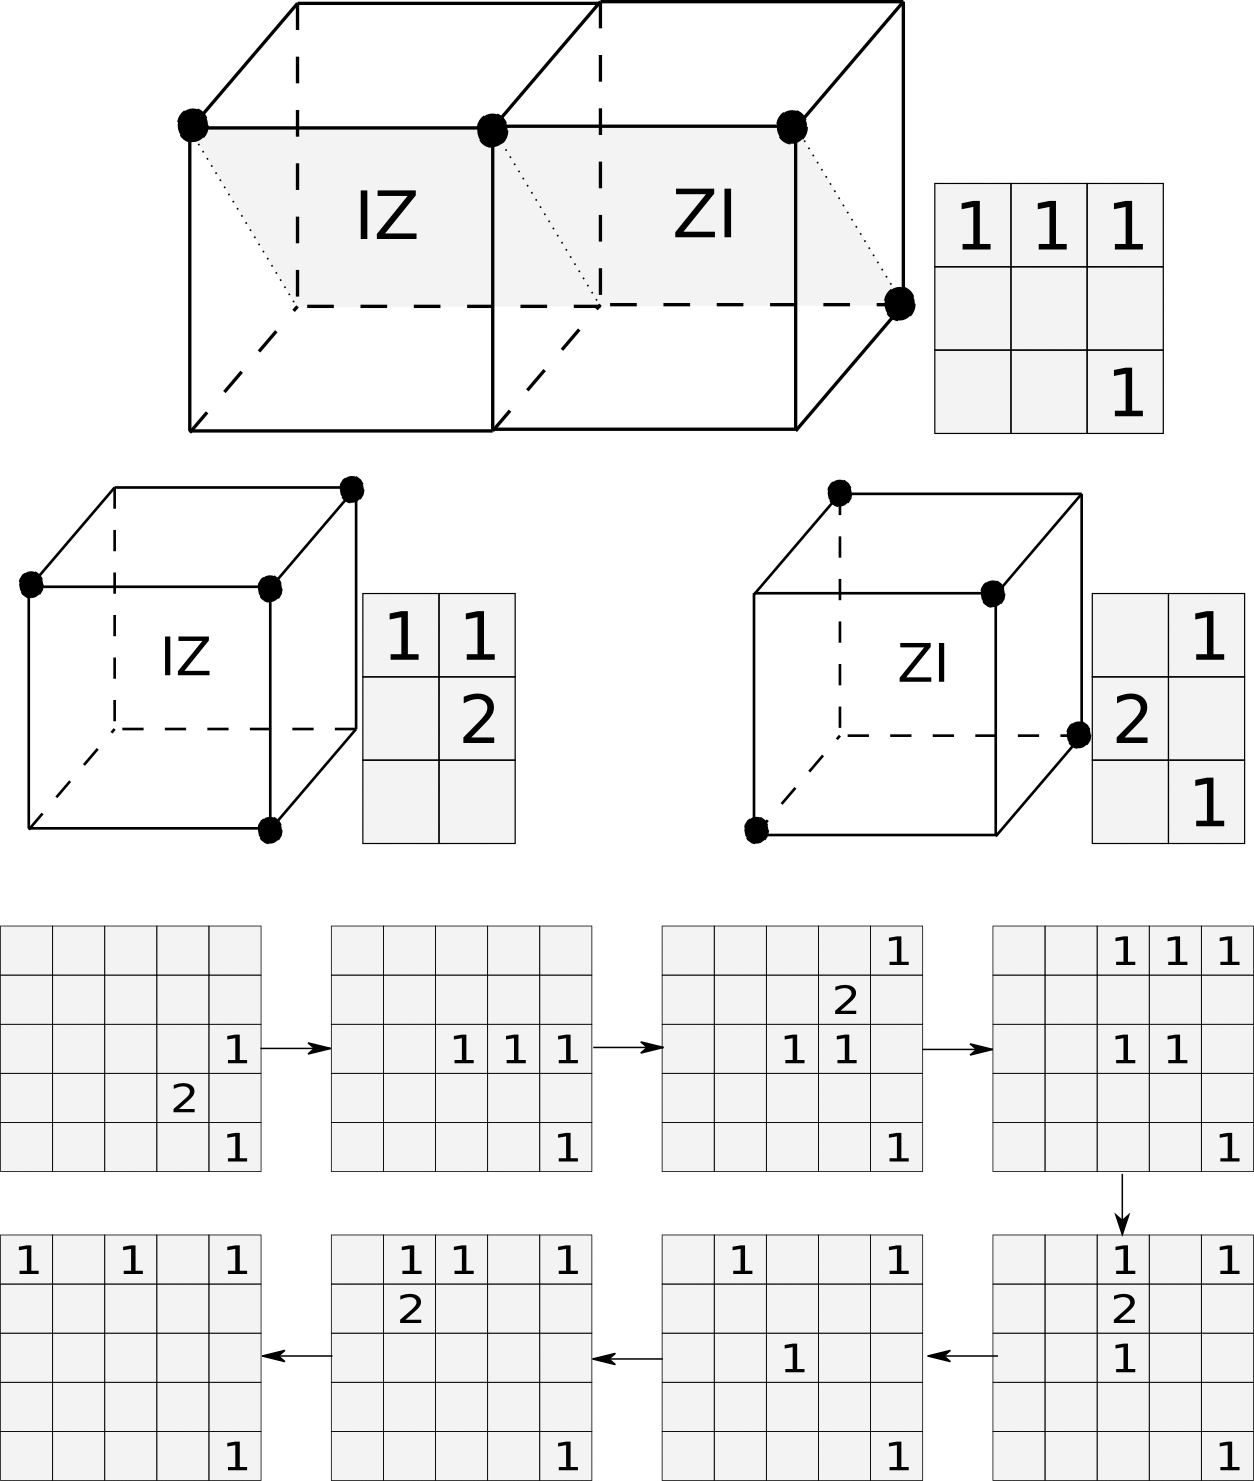
\includegraphics[width=.5\textwidth]{hook}
\caption{Construction of a hook of level 2 from the vacuum.
The grid diagram represents the position and the number of defects in the ($x=z$)-plane.
For each transition, an operator of weight 1 is applied.
The total number of defects never exceeds 6.
From a level-$0$ hook (the second diagram in the sequence),
a level-$1$ hook (the last in the sequence) is constructed using extra 2 defects.}
\label{fig:hook}
\end{figure}

Indeed, we can illustrate explicitly an error path that separates 
a single defect from the rest by distance $2^p$ during which only $2p+4$ defects are needed.
Consider an error of weight 2 that creates 4 defects as shown in the top of Fig.~\ref{fig:hook}.
We call it the {\em level-0 hook}.
The bottom sequence depicts a process to create a configuration shown at the bottom-left,
which we call {\em level-1 hook}. 
One sees that level-$1$ hook is similar with ratio 2 to level-$0$, 
and is obtained from level-0 with extra 2 defects.
One defines level-$p$ hooks hierarchically.
We claim that a level-$p$ hook can be constructed from the vacuum using $2p+4$ defects.
The proof is by induction.
The case $p=1$ is treated in the diagrams.
Suppose we can construct level-$p$ hook using $2p+4$ defects.
Consider the $2^{nd}$, $4^{th}$, $6^{th}$, and $8^{th}$ steps in Fig.~\ref{fig:hook}.
They can be viewed as a minuscule version of level-$p$ steps 
that construct a level-$(p+1)$ hook from the level-$p$ hooks. 
It requires at most $2p+4+2$ defects to perform the level-$p$ step; 
this completes the induction.

It may not be obvious whether a high level hook corresponds to a nontrivial logical operator,
but such a large hook is bad enough to make our decoder to fail.
